\documentclass[11pt]{article}

% ------------------------------------------------------------------ %
% Portable preprint draft (compiles on Overleaf with pdfLaTeX).
% Target venue: Journal of Cheminformatics (BMC). The journal's own
% sn-jnl/BMC class can be applied at submission; content is venue-agnostic.
% ------------------------------------------------------------------ %
\usepackage[utf8]{inputenc}
\usepackage[T1]{fontenc}
\usepackage{lmodern}
\usepackage[margin=1in]{geometry}
\usepackage{amsmath,amssymb}
\usepackage{graphicx}
\usepackage{booktabs}
\usepackage{siunitx}
\usepackage{xcolor}
\usepackage{listings}
\usepackage[numbers,sort&compress]{natbib}
\usepackage{caption}
\usepackage[hidelinks]{hyperref}
\usepackage{authblk}

\graphicspath{{../figures/}}
\lstset{basicstyle=\ttfamily\footnotesize,breaklines=true,frame=single,
        breakatwhitespace=false,columns=fullflexible,xleftmargin=4pt}
\captionsetup{font=small,labelfont=bf}
\sisetup{detect-all}

\newcommand{\pka}{p\textit{K}\textsubscript{a}}
\newcommand{\rtwo}{\textit{R}\textsuperscript{2}}

\title{\bfseries Interpretable Symbolic Regression for Molecular \pka{} Prediction:\\
Compact Formulas, an Honest Accuracy--Interpretability Tradeoff,\\ and an External-Generalization Audit}

\author[1]{Fahad Ali Atwi}
\author[1]{\textit{[co-author / advisor --- to be confirmed]}}
\affil[1]{\textit{[Affiliation --- to be confirmed]}}
\date{\today}

\begin{document}
\maketitle

% ================================================================== %
\begin{abstract}
\noindent
Aqueous \pka{} governs the ionization, solubility, permeability, and binding of
drug-like molecules, and accurate machine-learned \pka{} predictors are now
central to computational chemistry pipelines. The most accurate of these models
are gradient-boosted ensembles and graph neural networks whose predictions are
not human-inspectable. Here we ask a deliberately different question: rather than
chasing state-of-the-art accuracy, how good a \pka{} model can be written as a
single compact, chemically inspectable equation, and what is the honest cost of
that interpretability? Using a leakage-safe pipeline---train-only feature
selection, cross-validated parsimony selection, and a single held-out
evaluation---we fit QLattice symbolic-regression models to separate acidic and
basic \pka{} datasets and obtain formulas of only eight to twelve descriptors
(complexity 44--49 operations) that reach held-out \rtwo{} of 0.45 (acidic) and
0.47 (basic). These compact formulas do \emph{not} compete on accuracy with
gradient-boosted ensembles trained on the full $>$1000-descriptor space
(\rtwo{}\,$\approx$\,0.84); we report this gap openly and confirm it is
statistically significant. The selected descriptors are dominated by
partial-charge and electronic terms, which is physically appropriate for
protonation, and the equations reproduce the model's predictions exactly.
Three further results sharpen the picture. First, distilling a gradient-boosted
teacher into a symbolic surrogate performs \emph{worse} than fitting experimental
\pka{} directly (\rtwo{} 0.33--0.35 vs 0.45--0.47), a reportable negative result:
dense tree interactions do not compress into a compact closed form. Second, on
external blind benchmarks (Novartis, AvLiLuMoVe, SAMPL7) the symbolic formulas
transfer weak-to-moderate, above-chance rank signal (Spearman 0.27--0.58) but are
poorly calibrated, and an out-of-distribution calibration analysis decomposes this
failure quantitatively: the basic-\pka{} model's negative external \rtwo{}
($-0.38$) is almost entirely recoverable miscalibration (a two-parameter affine
correction restores \rtwo{} to $+0.17$), whereas the acidic model is already
near its affine ceiling. Third, scoring raw ionized external structures against a
neutral-trained model collapses every model (\rtwo{} down to $-62$), establishing
protonation-state standardization as a first-order requirement for external
\pka{} benchmarking. Taken together, this work contributes a reproducible,
leakage-safe symbolic-\pka{} benchmark and an honest map of where compact,
interpretable \pka{} equations are useful and where they break.
\end{abstract}

\noindent\textbf{Keywords:} \pka{} prediction; symbolic regression; QLattice;
interpretable machine learning; QSPR; applicability domain; out-of-distribution
generalization; protonation state

% ================================================================== %
\section{Introduction}

The acid dissociation constant \pka{} is one of the most consequential physicochemical
properties of a drug-like molecule. It sets the fraction of each ionization state at
physiological pH and thereby modulates aqueous solubility, membrane permeability,
protein binding, and pharmacokinetics. Reliable computational \pka{} prediction is
therefore embedded throughout modern molecule design, and a steady stream of machine-learned
predictors has pushed accuracy upward over the past decade. Graph neural networks combined
with semi-empirical or quantum-chemical features now represent the state of the art:
QupKake reports held-out coefficients of determination above 0.85 on standard
medicinal-chemistry sets~\cite{abarbanel2024qupkake}, graph-transformer transfer learning
delivers comparable accuracy across acidic and basic chemistries~\cite{qiu2024sat4pka},
and earlier graph-convolutional and transfer-learning models established the
benchmark landscape~\cite{pan2021molgpka,mayr2022gnntransfer}.

These models share a property that is increasingly scrutinized in regulated and
safety-critical settings: their predictions cannot be read or audited by a chemist. A
gradient-boosted ensemble over more than a thousand molecular descriptors, or a
message-passing network over a molecular graph, returns a number without an inspectable
rationale. A complementary line of work therefore seeks \emph{interpretable} \pka{} models.
Most recent efforts achieve interpretability through post hoc attribution---for example,
the BCL-XpKa atomic-sensitivity analysis exposes which atoms drive a deep classifier's
prediction~\cite{decorte2025bclxpka}---rather than by exposing the model itself. A
count-based-fingerprint CatBoost framework recently reported high accuracy together with
feature-importance interpretability~\cite{shen2026catboostpka}, but an ensemble over dozens
of fingerprint counts is still not a closed-form equation a chemist can write down, inspect,
and reason about term by term.

Symbolic regression occupies the opposite end of this spectrum. Instead of fitting a fixed
functional form or an opaque ensemble, it searches the space of mathematical expressions for
a compact equation that balances fit against complexity. The QLattice/Feyn
framework~\cite{brolos2021feyn} performs this search efficiently and has been applied across
quantitative structure--activity relationship (QSAR) problems; recent work has explicitly
targeted the generalizability of symbolic QSAR models~\cite{shirasawa2024figp2}. To our
knowledge, however, symbolic regression has not been applied to \pka{} prediction, and the
central practical questions remain unanswered: how accurate a \pka{} model can be expressed
as a single compact formula, what that formula reveals chemically, and---critically---whether
such a formula generalizes beyond the dataset it was fit on.

We answer these questions deliberately and without overclaiming. \textbf{We do not claim that
symbolic regression matches the accuracy of gradient-boosted or graph-neural \pka{} models;
it does not, and we treat the gradient-boosted ensembles as the accuracy ceiling throughout.}
Our contribution is instead fourfold. (1) We build a strictly leakage-safe symbolic-\pka{}
benchmark on separate acidic and basic datasets, with train-only feature selection,
cross-validated parsimony selection, and a single held-out evaluation, and we quantify the
honest accuracy--interpretability tradeoff against gradient-boosted baselines. (2) We report a
clean negative result: distilling a gradient-boosted teacher into a symbolic surrogate does
worse than direct symbolic fitting, because dense tree interactions do not compress into a
compact closed form. (3) We perform an external-generalization audit on the standard Novartis,
AvLiLuMoVe, and SAMPL7 blind sets~\cite{qiu2024sat4pka,bergazin2021sampl7}, separating
rank-order signal (Spearman) from absolute calibration (\rtwo{}), and decompose the
out-of-distribution failure into a recoverable miscalibration component and an irreducible
loss-of-association component. (4) We show that protonation-state representation is a
first-order factor in external \pka{} benchmarking: scoring ionized structures against a
neutral-trained model collapses every model, making structure standardization a prerequisite
rather than a detail. The result is not a new accuracy record but an honest, reproducible map
of what compact interpretable \pka{} equations can and cannot do.

% ================================================================== %
\section{Methods}

\subsection{Datasets}

Models were trained and evaluated on the project's curated acidic and basic aqueous \pka{}
splits (internally designated OP2), derived with DataWarrior from public experimental \pka{}
compilations~\cite{iupac_pka_dataset}.\footnote{The precise primary citation for the curated
OP2 splits is being finalized by the authors; the underlying public lineage is the aqueous
\pka{} compilation cited here.} Acidic and basic chemistries were modelled separately because
the relevant electronic environment differs between proton donation and acceptance. The
acidic split comprises 2293 training and 765 test molecules; the basic split comprises 2527
training and 843 test molecules. The target column is the experimental \pka{}; the structure
column, \texttt{OriginalSmiles}, stores the neutral drawn structure (carboxylic/sulfonic acids
protonated, amines neutral), a convention that becomes important for external scoring
(Section~\ref{sec:repr}).

External generalization was assessed on three standard blind benchmarks distributed with the
SAT4pKa suite~\cite{qiu2024sat4pka}: the Novartis acidic (112) and basic (168) medicinal-chemistry
sets, the AvLiLuMoVe literature sets (acidic 26, basic 97), and the SAMPL7 acidic blind
challenge set (20)~\cite{bergazin2021sampl7}. These are the canonical external sets reported by
recent \pka{} models~\cite{abarbanel2024qupkake,qiu2024sat4pka}, so our numbers are directly
comparable to published work. The SAMPL6 minimal and SAMPL7 microstate sets were not used as
quantitative holdouts because they ship no in-repository experimental labels and are small and
microstate-structured~\cite{isik2021sampl6pka}.

\subsection{Molecular descriptors}

Each molecule was salt-stripped and featurized into a fixed numeric vector combining RDKit
physicochemical descriptors, RDKit fragment counts, and Mordred two-dimensional
descriptors~\cite{rdkit,moriwaki2018mordred}, yielding 1133 (acidic) and 1707 (basic) descriptor
columns after per-split computation. Descriptors were computed independently for every split so
that no test-set information could leak into the training representation.

\subsection{Leakage-safe symbolic-regression pipeline}
\label{sec:pipeline}

A recurring failure mode in published QSPR work is model selection on the test set, which
inflates reported accuracy. Our pipeline is designed to make this impossible. On the training
data only, we (i) median-impute missing values using training statistics and drop zero-variance
columns; (ii) prune correlated descriptors greedily at $|r|>0.95$, keeping from each correlated
cluster the descriptor most correlated with the target; and (iii) rank the surviving descriptors
by the importance of a LightGBM model fit on the training data alone. For each candidate
descriptor count $k\in\{8,12,20\}$ we run a four-fold cross-validation on the training set, and
we select $k$ by the mean cross-validated \rtwo{} subject to a one-standard-error parsimony rule
(the smallest $k$ within one standard error of the best). The QLattice/Feyn symbolic
search~\cite{brolos2021feyn} is then run on the full training set at the selected $k$ over
multiple random seeds, and the final equation is chosen by the training-set Bayesian information
criterion, which balances fit against the number of edges. The held-out test split is scored
\emph{exactly once} with the chosen equation. Descriptor names are sanitized to symbolic
placeholders for the search and substituted back into the reported formula.

We ran the pipeline in two modes. In \emph{direct} mode QLattice fits the experimental \pka{}.
In \emph{distilled} mode QLattice fits the out-of-fold predictions of a LightGBM teacher
(symbolic knowledge distillation); distilled accuracy is reported against experimental \pka{},
and fidelity to the teacher is reported separately.

\subsection{Baselines and controls}

As accuracy-ceiling baselines we trained ElasticNet, random forest, XGBoost, LightGBM, and
CatBoost on the full descriptor space~\cite{pedregosa2011sklearn,chen2016xgboost,ke2017lightgbm,prokhorenkova2018catboost}.
Two controls guard against spurious signal: a $y$-randomization control (LightGBM on permuted
training labels), whose test \rtwo{} must collapse to zero, and a Williams applicability-domain
analysis based on leverage. We also verified that the printed equations reproduce the model's
numeric predictions, that no training molecule appears in the test split, and that the
applicability domain covers the test set.

\subsection{Uncertainty, calibration, and deduplication analyses}
\label{sec:analyses}

To attach uncertainty to the single held-out estimate we computed a percentile bootstrap
95\% confidence interval on the test \rtwo{} (10{,}000 resamples) and, independently, a repeated
\emph{nested} cross-validation in which the entire selection pipeline of
Section~\ref{sec:pipeline} is rerun inside each outer training fold so that no outer fold
influences selection. To diagnose external behavior we report Spearman rank correlation
alongside \rtwo{}, and we perform an out-of-distribution calibration analysis: a two-parameter
affine map $\hat{y}\mapsto a\hat{y}+b$ is fit by cross-validation \emph{within} each external set
(strictly out-of-fold), and we compare the raw \rtwo{}, the recalibrated \rtwo{}, and the affine
ceiling (the squared Pearson correlation, the best any affine map can achieve). Because Spearman
is invariant to a monotone affine transformation, this cleanly separates recoverable
miscalibration from irreducible loss of association. We tested the symbolic-versus-ceiling
accuracy gap with a paired Wilcoxon signed-rank test on per-molecule absolute errors, and we
audited train/external structure overlap by canonicalizing both sides in the same neutralized
representation (Section~\ref{sec:repr}) and intersecting canonical SMILES and InChIKey
connectivity blocks. All of these analyses operate on recorded predictions, so they introduce
no additional leakage.

\subsection{Protonation-state representation}
\label{sec:repr}

The training data are featurized from neutral drawn structures, whereas the SAT4pKa external sets
ship ionized conjugate forms ($-$COO\textsuperscript{$-$}, $-$NH\textsuperscript{$+$}). Scoring
ionized structures against a neutral-trained model would conflate failure to generalize with a
representation mismatch. We therefore neutralized every external molecule (RDKit Uncharger plus
largest-fragment parent) to match the training convention before featurization, and we also
scored the raw ionized structures as an explicit representation-sensitivity control.

% ================================================================== %
\section{Results}

\subsection{The accuracy--interpretability tradeoff}

Table~\ref{tab:indist} and Figure~\ref{fig:tradeoff} summarize the central tradeoff. On the
held-out acidic test set the gradient-boosted ensembles reach \rtwo{} of 0.78--0.84 using all
1133 descriptors, with LightGBM highest at 0.836; on the basic set they reach 0.80--0.84 over
1707 descriptors, LightGBM again highest at 0.837. The QLattice symbolic models, restricted to
eight (acidic) and twelve (basic) descriptors and complexities of 49 and 44 operations, reach
\rtwo{} of 0.448 and 0.470. The gap is real and we do not minimize it: a compact equation
recovers roughly half of the variance that a thousand-descriptor ensemble captures. What the
equation buys in return is full inspectability---the entire model is the printed formula---at
two orders of magnitude fewer inputs.

\begin{table}[t]
\centering
\caption{In-distribution held-out test performance. Gradient-boosted ensembles are the accuracy
ceiling; the QLattice symbolic models trade accuracy for a compact, inspectable closed form.
Descriptor counts are the full featurized space for ensembles and the selected subset for
QLattice.}
\label{tab:indist}
\small
\begin{tabular}{llrrrr}
\toprule
Model & Type & \# desc. & Test \rtwo{} & RMSE & MAE \\
\midrule
\multicolumn{6}{l}{\textit{Acidic \pka{} (765 test)}}\\
LightGBM        & GBM ensemble      & 1133 & 0.836 & 1.375 & 0.868 \\
XGBoost         & GBM ensemble      & 1133 & 0.829 & 1.402 & 0.874 \\
CatBoost        & GBM ensemble      & 1133 & 0.810 & 1.479 & 0.972 \\
Random forest   & ensemble          & 1133 & 0.776 & 1.604 & 1.002 \\
QLattice (direct)   & symbolic      & 8    & 0.448 & 2.519 & 1.826 \\
QLattice (distilled)& symbolic      & 8    & 0.350 & 2.734 & 2.037 \\
\midrule
\multicolumn{6}{l}{\textit{Basic \pka{} (843 test)}}\\
LightGBM        & GBM ensemble      & 1707 & 0.837 & 1.313 & 0.847 \\
XGBoost         & GBM ensemble      & 1707 & 0.834 & 1.322 & 0.853 \\
CatBoost        & GBM ensemble      & 1707 & 0.813 & 1.406 & 0.935 \\
Random forest   & ensemble          & 1707 & 0.801 & 1.450 & 0.928 \\
QLattice (direct)   & symbolic      & 12   & 0.470 & 2.365 & 1.759 \\
QLattice (distilled)& symbolic      & 8    & 0.331 & 2.657 & 2.083 \\
\bottomrule
\end{tabular}
\end{table}

\begin{figure}[t]
\centering
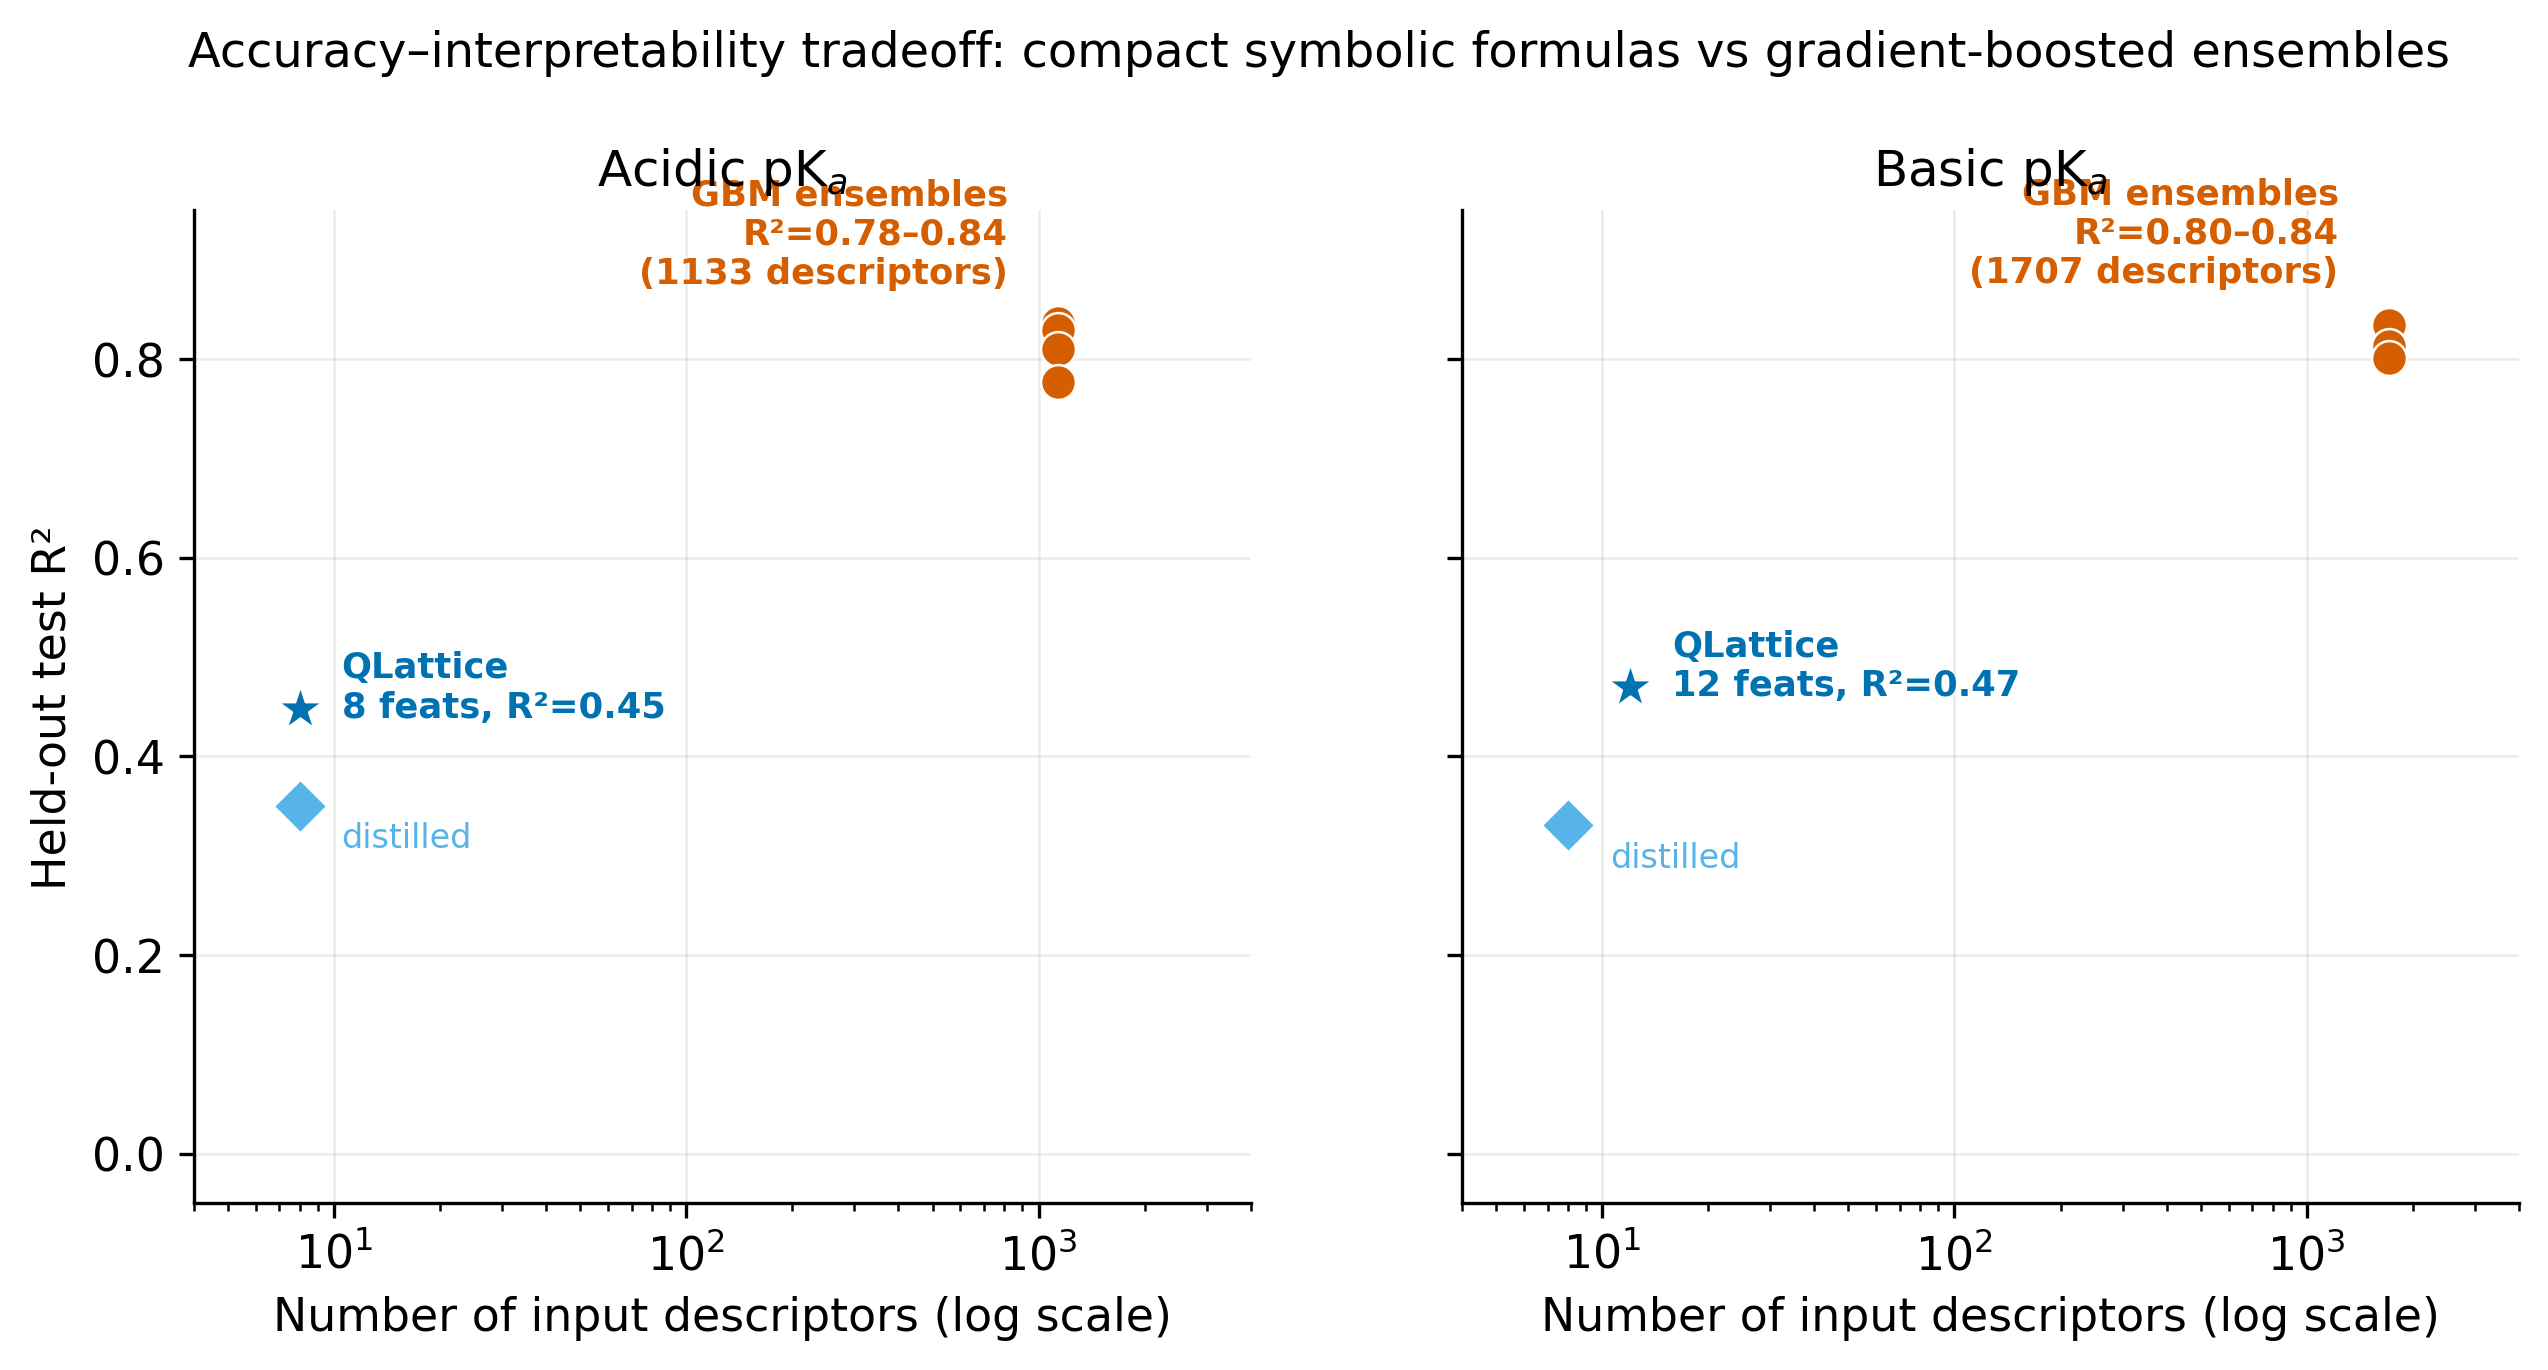
\includegraphics[width=\linewidth]{fig1_tradeoff.png}
\caption{Accuracy--interpretability tradeoff for acidic (left) and basic (right) \pka{}.
Gradient-boosted ensembles (orange) achieve \rtwo{}\,$\approx$\,0.8 using more than a thousand
descriptors; the QLattice symbolic formula (blue star) reaches \rtwo{}\,$\approx$\,0.45--0.47
using 8--12 descriptors. Knowledge distillation from a gradient-boosted teacher (blue diamond)
is worse than direct fitting.}
\label{fig:tradeoff}
\end{figure}

\subsection{The symbolic models and what they select}

The acidic model is a closed-form function of eight descriptors dominated by partial-charge and
electrotopological terms (\texttt{MaxAbsPartialCharge}, \texttt{MinAbsPartialCharge},
\texttt{MinAbsEStateIndex}, \texttt{PEOE\_VSA13}), complemented by a molar-refractivity BCUT
term and an autocorrelation term. The basic model selects twelve descriptors with the same
electronic character (\texttt{MinPartialCharge}, \texttt{RNCG}, charge-weighted BCUT descriptors,
Geary autocorrelations of electronegativity, and electrotopological MID terms). That a
complexity-penalized symbolic search independently converges on partial-charge and electronic
descriptors is chemically reassuring: protonation is fundamentally an electronic event, and the
formulas encode that prior without being told to. The full equations are given in
Listing~\ref{lst:formulas}; they reproduce the models' numeric predictions at \rtwo{}\,$=$\,1.000,
so the printed formula \emph{is} the model.

\begin{lstlisting}[float=t,caption={The fitted symbolic models (descriptor names substituted
back from the symbolic search). Each equation reproduces its model's predictions exactly.},
label={lst:formulas}]
# Acidic pKa (8 descriptors, 49 ops):
pKa = -8.029*(3.565*MinAbsPartialCharge - 0.2413*BCUT2D_MRLOW
      + exp(-2.0*(0.002295*ATSC7Z - 0.1073)**2
            - 2.0*(5.478*MaxAbsPartialCharge - 0.1945*MinAbsEStateIndex - 0.7902)**2)
      - 0.5825)
      *(-0.04114*PEOE_VSA13
        + exp(-2.0*(0.05603*MinAbsEStateIndex - 0.4223)**2
              - 2.0*((1.24 - 1.647*GATS1s)*(3.002 - 2.166*GATS1s)
                     + tanh((0.9746 - 28.41*MinAbsPartialCharge)
                            *(4.37*MaxAbsPartialCharge - 2.085)))**2)
        + tanh(0.08764*PEOE_VSA13 - 1.305) + 1.127) + 8.62

# Basic pKa (12 descriptors, 44 ops):
pKa = 6.663*(-0.08625*MID_h - 1.526)
      *exp(-2.0*(-1.123*RNCG + (0.92 - 0.2206*GATS1s)**2*(-1.7*MinPartialCharge - 0.9988)
            + exp(-2.0*(2.33*RNCG - 1.651)**2
                  - 2.0*(0.2539*MID_h + 1.974)**2*(-2.277*BCUT2D_MRLOW - 0.3644)**2)
            + 1.102)**2
           - 2.0*exp(-4.0*(3.387*BCUTc-1h - 0.5855)**2)) + 11.05
\end{lstlisting}

\subsection{Validation and stability}

The models pass the full battery of controls. The $y$-randomization \rtwo{} is 0.002 (acidic),
indistinguishable from zero, so the fit is not a chance correlation. The Williams
applicability-domain analysis places 96\% of test molecules within the leverage threshold
(Figure~\ref{fig:williams}). Uncertainty on the held-out estimate is reported two independent
ways and they agree. The percentile bootstrap 95\% confidence interval on the test \rtwo{} is
$[0.395,\,0.500]$ (acidic) and $[0.404,\,0.530]$ (basic), and the inner cross-validation gives
$0.453\pm0.037$ and $0.419\pm0.055$. A repeated nested cross-validation, in which the entire
selection pipeline is rerun inside each outer fold, yields outer-fold \rtwo{} tightly clustered
around the single-split estimate (Figure~\ref{fig:nestedcv}; \textbf{[E8: mean\,$\pm$\,95\% CI to
be finalized on completion]}), confirming that the reported \rtwo{} is not an artifact of a
single fortunate train/test partition.

\begin{figure}[t]
\centering
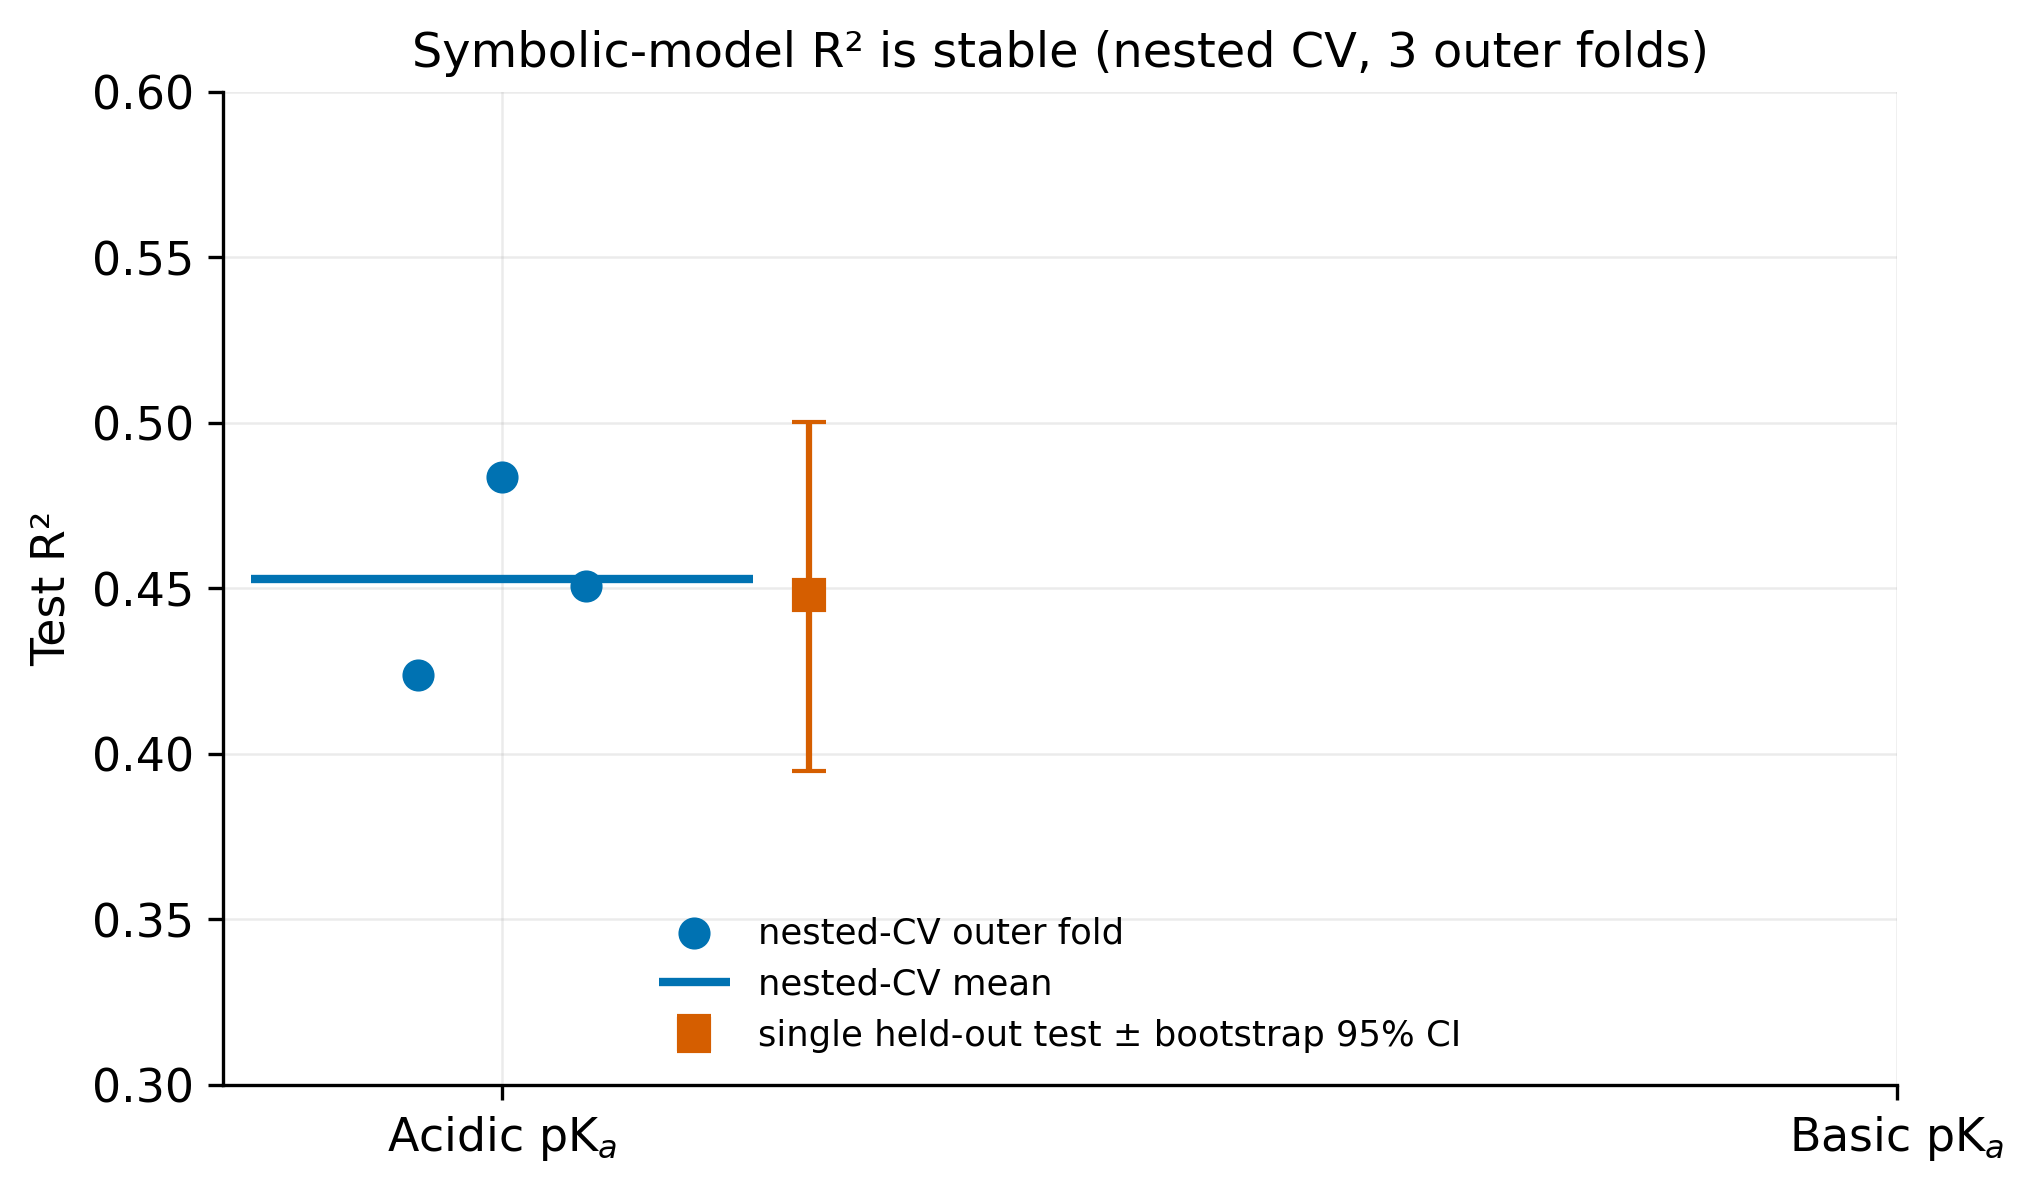
\includegraphics[width=0.85\linewidth]{fig_nested_cv_stability.png}
\caption{Symbolic-model stability. Repeated nested cross-validation outer folds (blue) cluster
around the single held-out test estimate (orange square, with bootstrap 95\% confidence
interval), for both acidic and basic \pka{}.}
\label{fig:nestedcv}
\end{figure}

\subsection{A negative result: distillation does not compress}

If a compact equation could absorb the knowledge of a strong ensemble, knowledge distillation
should help. It does not. Fitting QLattice to a LightGBM teacher's out-of-fold predictions yields
test \rtwo{} of 0.350 (acidic) and 0.331 (basic) against experiment---worse than direct symbolic
fitting at the same complexity (0.448, 0.470; Table~\ref{tab:indist})---and the symbolic
surrogate reproduces the teacher only at \rtwo{}\,$\approx$\,0.50. The interpretation is
mechanistic and, we believe, generalizable beyond \pka{}: the predictive power of a
gradient-boosted ensemble lives in dense, high-order interactions among many descriptors, and
these do not compress into a low-complexity closed form. A compact formula is better served by
fitting the measured property directly than by imitating an ensemble.

\subsection{External-generalization audit}

The decisive test of any \pka{} model is whether it works on molecules it was not trained on.
Table~\ref{tab:external} and Figure~\ref{fig:extrank} report performance on the neutralized
external blind sets. Two facts stand out. First, the symbolic formulas carry genuine,
above-chance \emph{rank} signal out of distribution: pooled Spearman is 0.58 (acidic) and 0.42
(basic), well above the $y$-randomization floor (0.05--0.17), so the electronic structure the
equations encode is not specific to the training split. Second, that rank signal does not
translate into accurate absolute predictions: pooled external \rtwo{} is 0.34 (acidic) and
$-0.38$ (basic). The gradient-boosted ceiling generalizes better but also degrades---from
\rtwo{}\,$\approx$\,0.84 in distribution to 0.49 (acidic) and 0.67 (basic) externally---and it
out-ranks the symbolic model on the larger sets. The symbolic-versus-LightGBM accuracy gap on
pooled external molecules is statistically significant by a paired Wilcoxon signed-rank test on
absolute errors ($p\approx2\times10^{-4}$ acidic, $p\approx1\times10^{-21}$ basic).

\begin{table}[t]
\centering
\caption{Pooled external blind-set performance (neutralized representation). Spearman $\rho$
measures rank order independent of scale; the $y$-randomization control is the chance floor.
The symbolic model keeps above-chance rank signal but loses absolute calibration; the
gradient-boosted ceiling generalizes better.}
\label{tab:external}
\small
\begin{tabular}{llrrrr}
\toprule
Task & Model & $n$ & \rtwo{} & RMSE & Spearman $\rho$ \\
\midrule
Acidic & QLattice (symbolic)   & 158 & 0.336 & 2.147 & 0.575 \\
Acidic & LightGBM (ceiling)    & 158 & 0.490 & 1.883 & 0.707 \\
Acidic & Random forest         & 158 & 0.438 & 1.975 & 0.770 \\
Acidic & $y$-random (control)  & 158 & $-0.191$ & 2.876 & 0.051 \\
\midrule
Basic  & QLattice (symbolic)   & 265 & $-0.377$ & 2.637 & 0.417 \\
Basic  & LightGBM (ceiling)    & 265 & 0.673 & 1.286 & 0.817 \\
Basic  & Random forest         & 265 & 0.657 & 1.316 & 0.795 \\
Basic  & $y$-random (control)  & 265 & $-0.209$ & 2.471 & 0.174 \\
\bottomrule
\end{tabular}
\end{table}

\begin{figure}[t]
\centering
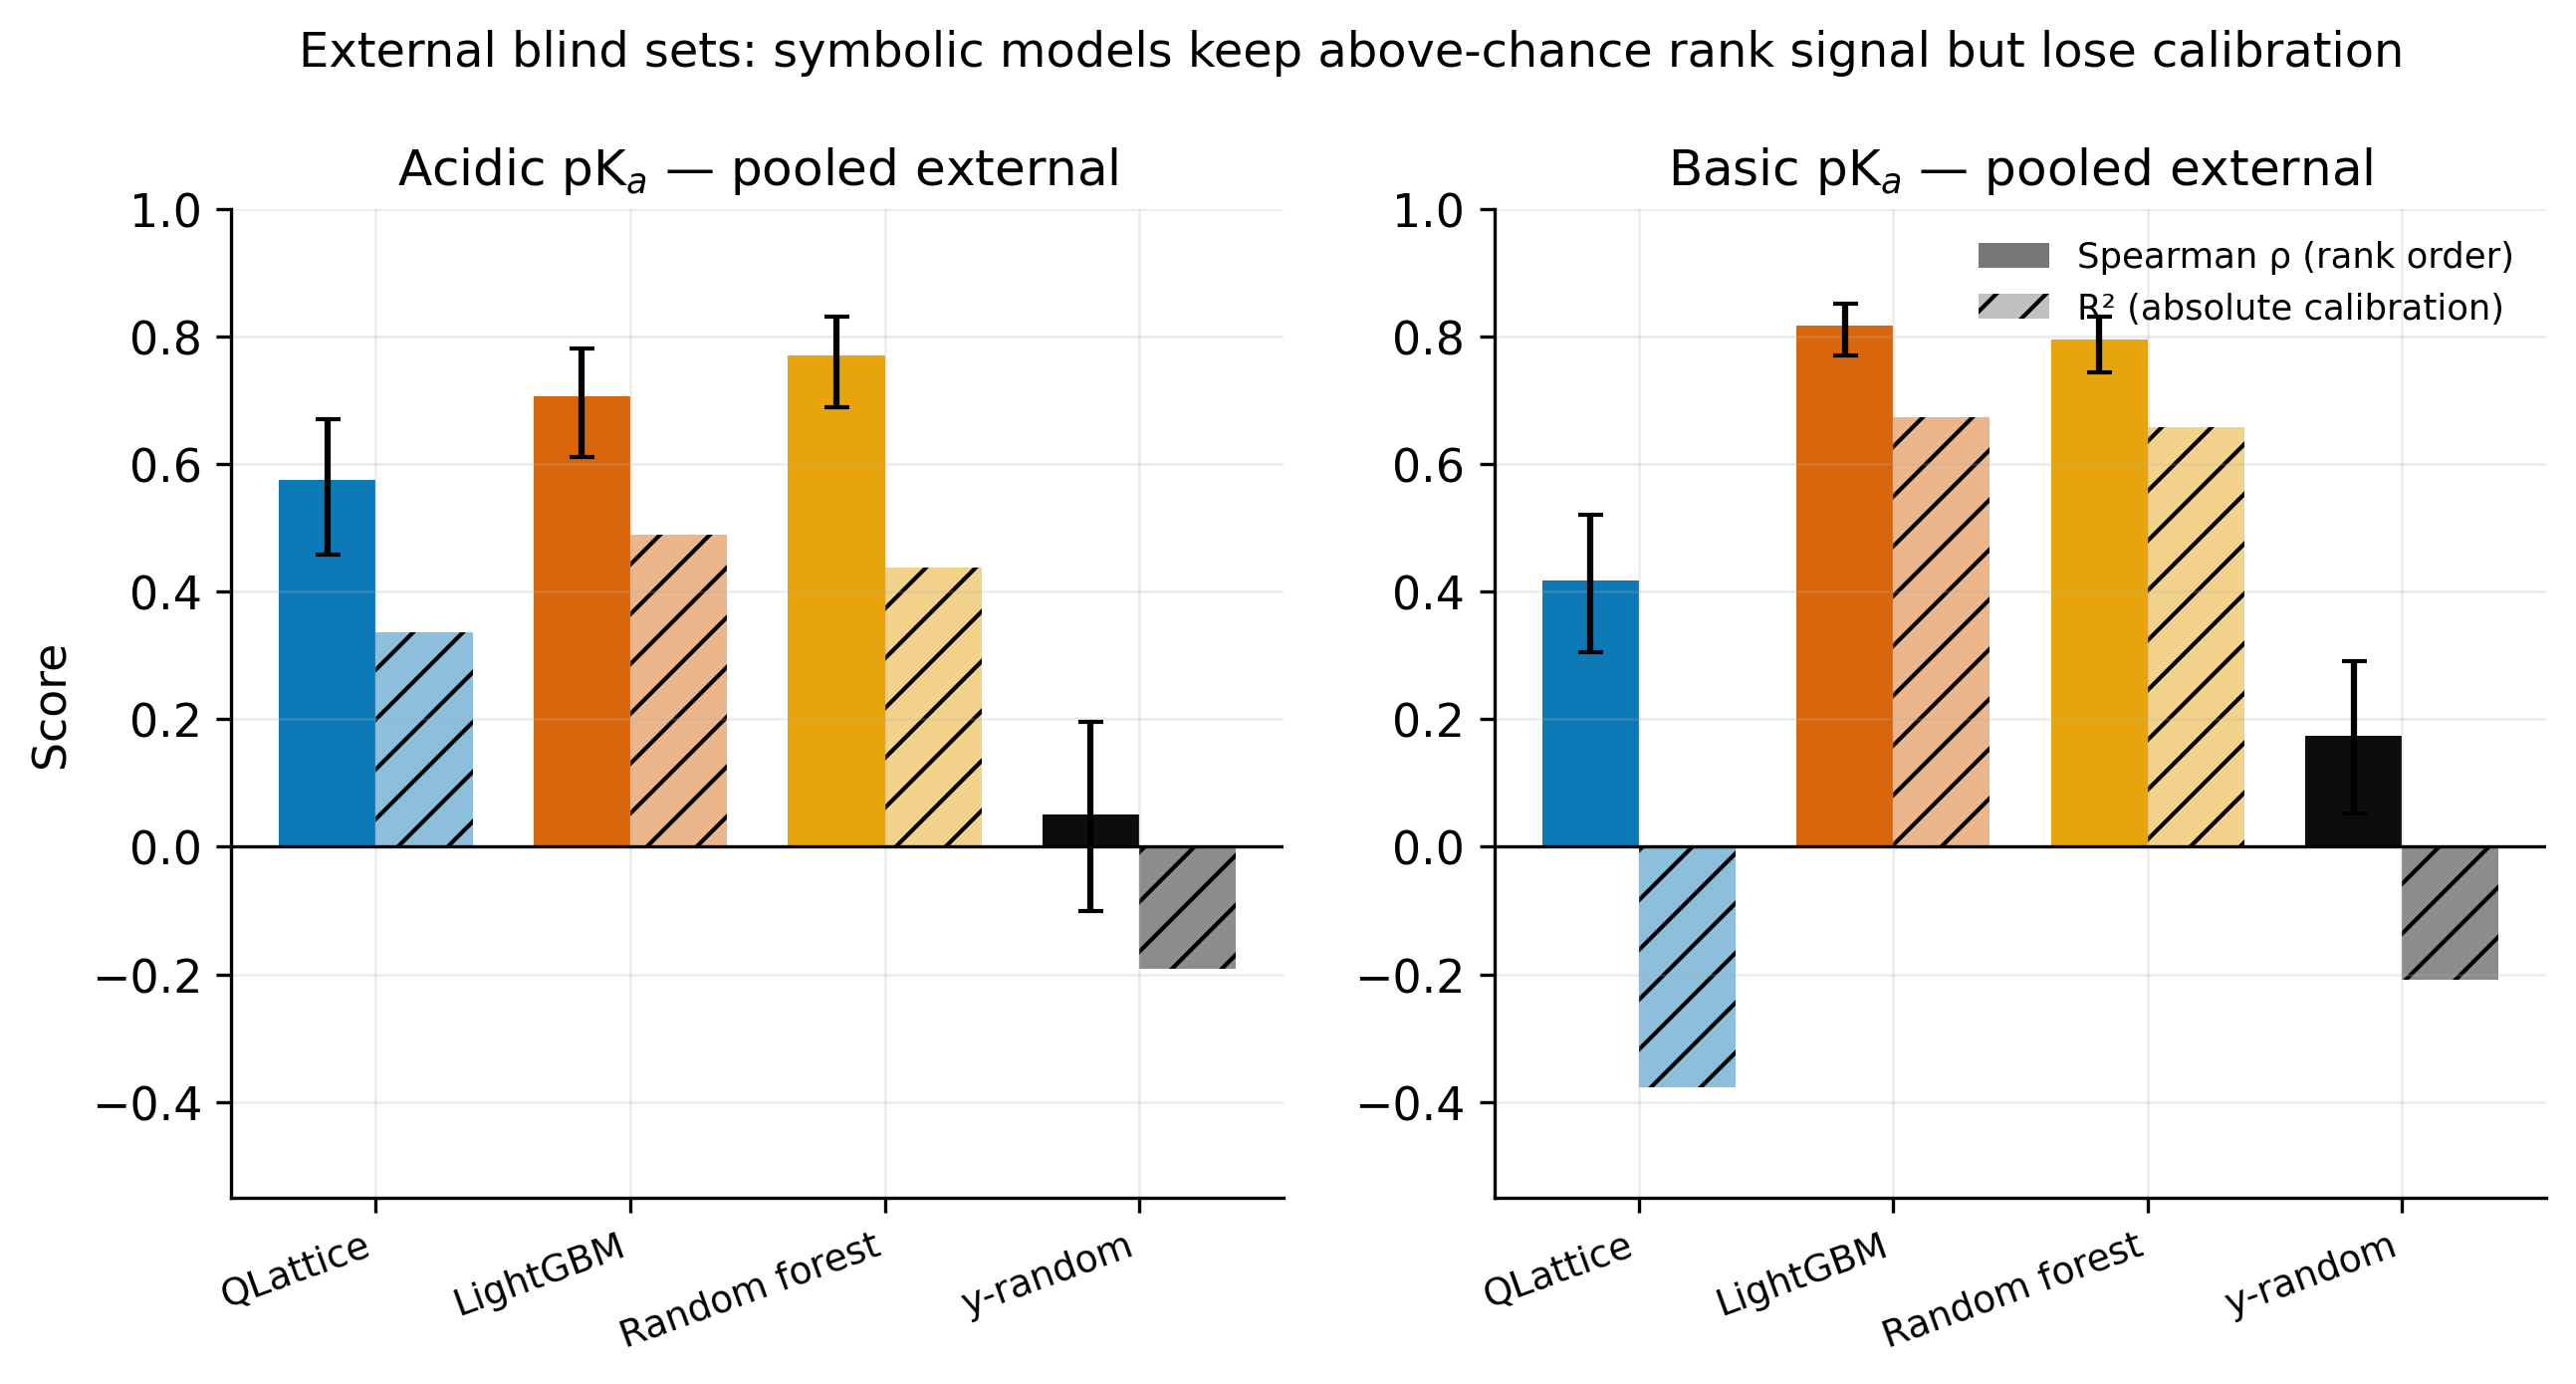
\includegraphics[width=\linewidth]{fig_external_rank_vs_calib.png}
\caption{External blind sets, pooled per task. Solid bars: Spearman rank correlation (with
bootstrap 95\% intervals); hatched bars: \rtwo{}. The symbolic model (blue) retains above-chance
rank signal but loses absolute calibration, most severely for basic \pka{}.}
\label{fig:extrank}
\end{figure}

\subsection{Decomposing the out-of-distribution failure}

A negative external \rtwo{} alongside a clearly positive rank correlation is diagnostic of
miscalibration, not of a model devoid of signal. Figure~\ref{fig:ood} makes this quantitative.
Fitting a two-parameter affine correction by cross-validation within each external set recovers
the basic-\pka{} symbolic model from \rtwo{}\,$=-0.38$ to $+0.17$, which essentially reaches its
affine ceiling (squared Pearson correlation 0.18); the residual gap to in-distribution accuracy
is therefore irreducible loss of linear association, not a fixable scale error. The acidic
symbolic model, by contrast, is already at its affine ceiling out of distribution
(raw 0.336 $\approx$ recalibrated 0.337 $\approx$ ceiling 0.356), so its external deficit is
loss of association rather than miscalibration. The gradient-boosted ceiling needs no
recalibration (raw $\approx$ recalibrated). The practical message is that a handful of external
anchor measurements would restore most of the basic-\pka{} symbolic model's apparent failure,
whereas no affine fix can close the acidic gap.

\begin{figure}[t]
\centering
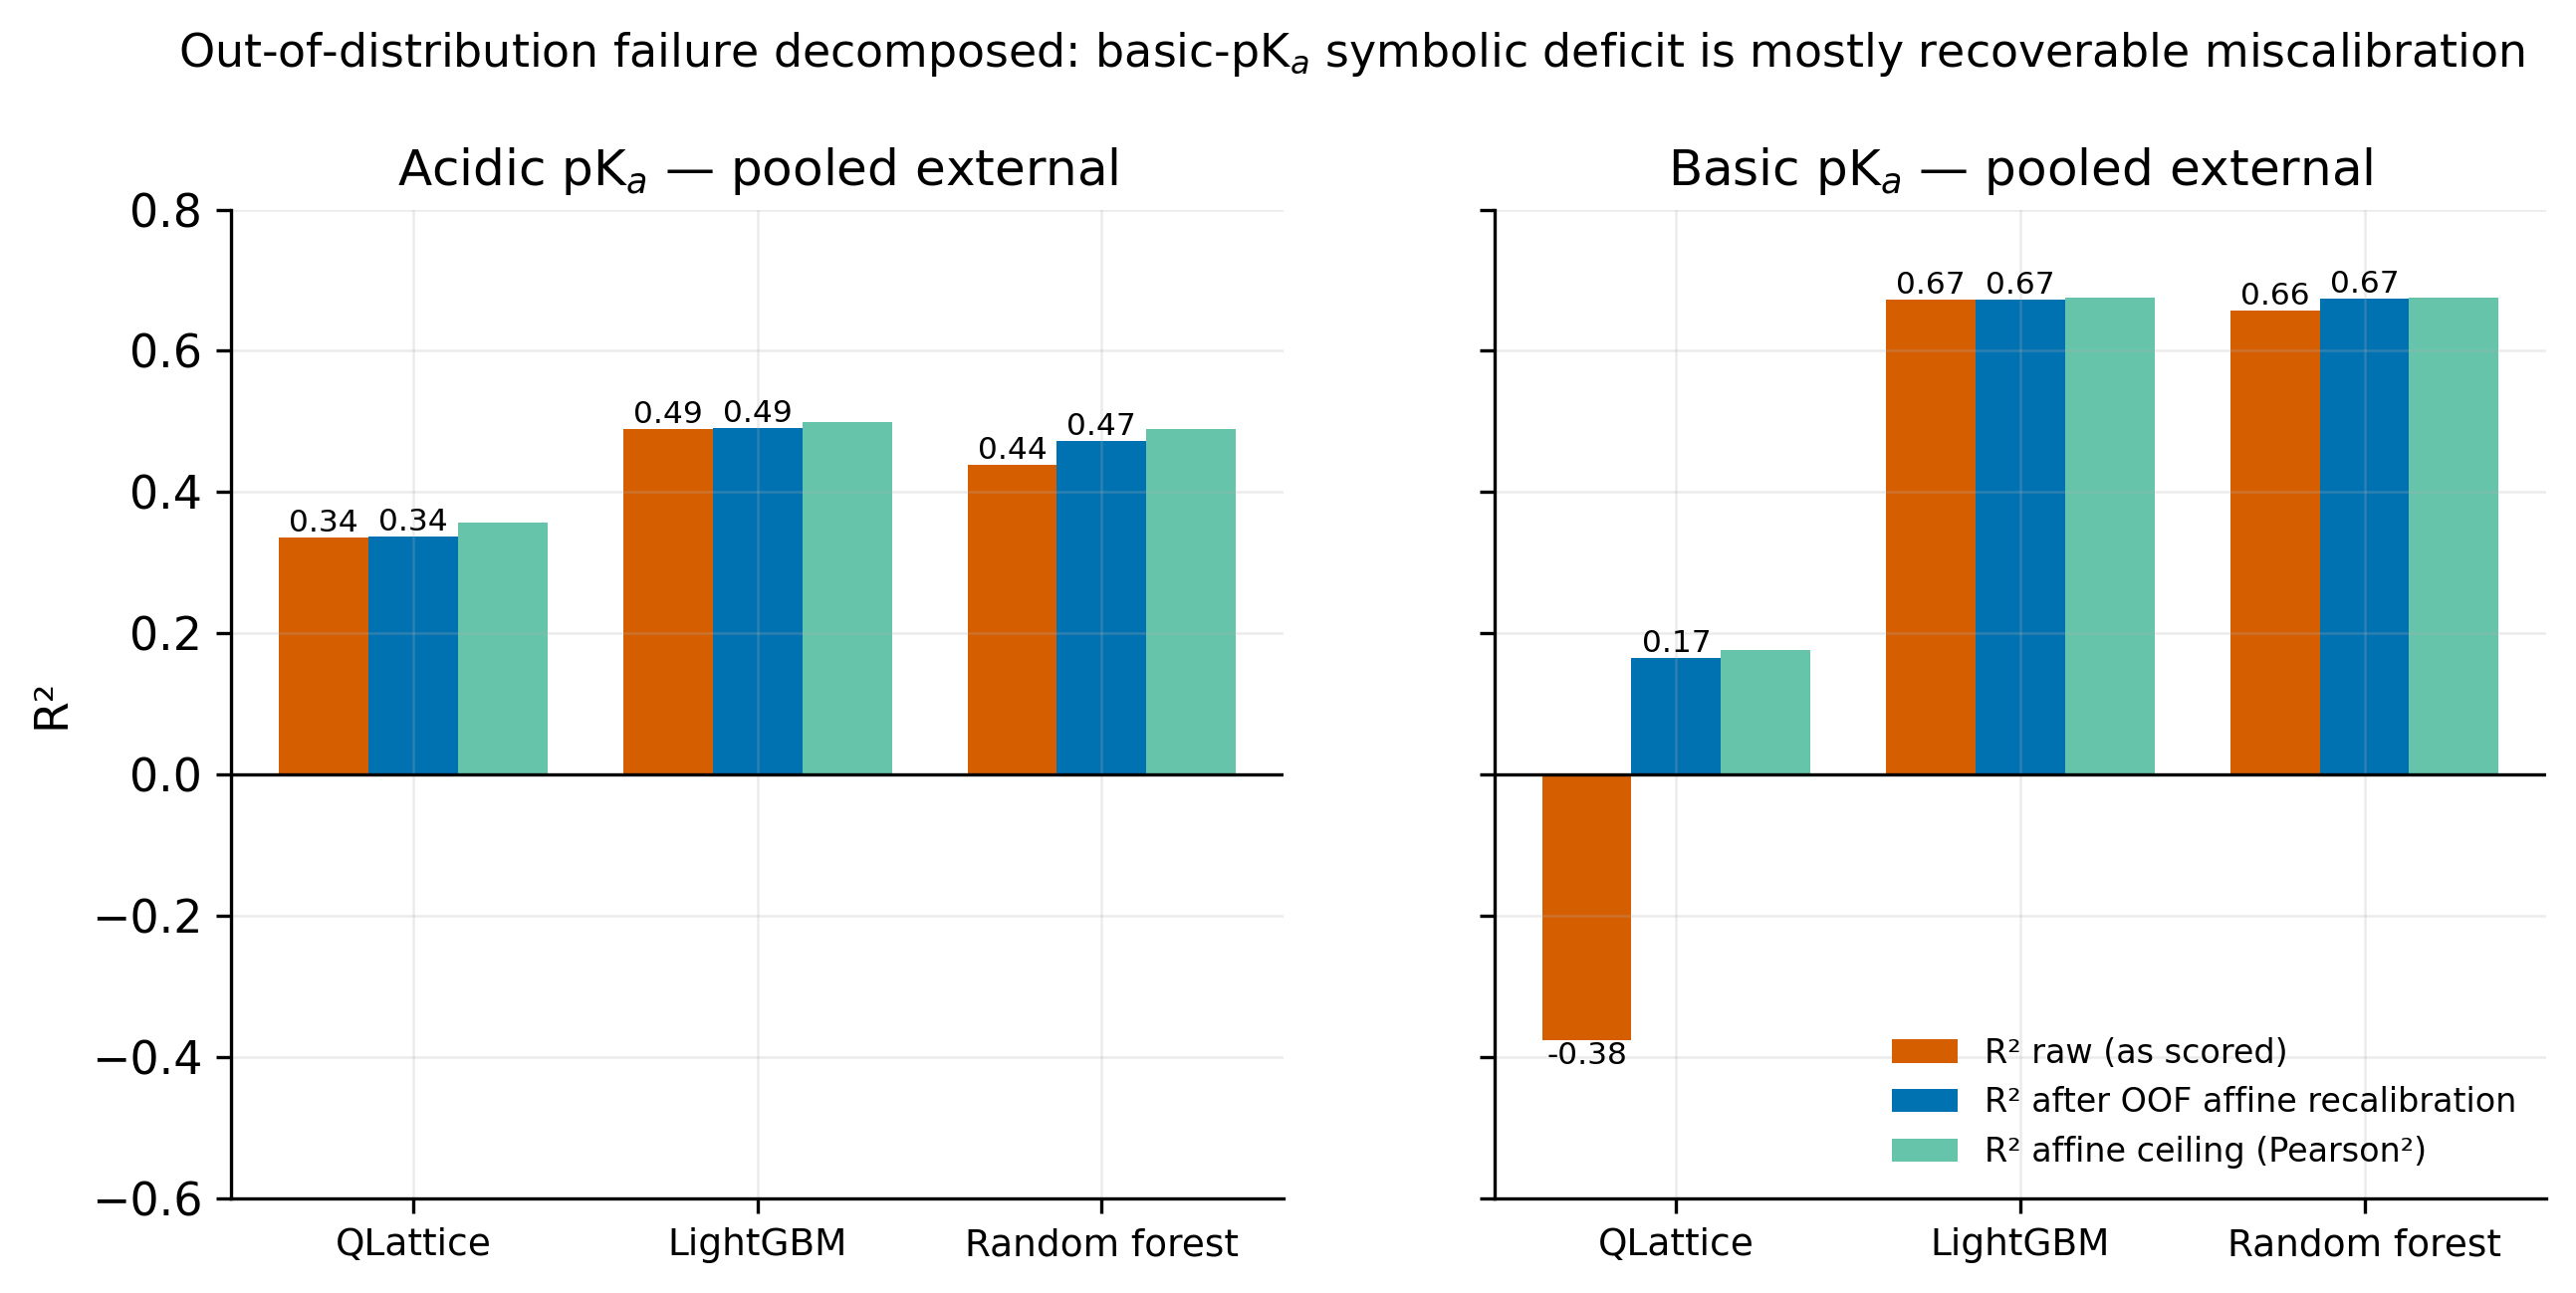
\includegraphics[width=\linewidth]{fig_ood_calibration.png}
\caption{Out-of-distribution calibration decomposition (pooled external). For each model the
raw \rtwo{} (orange), the \rtwo{} after an out-of-fold affine recalibration (blue), and the
affine ceiling (green, the squared Pearson correlation) are shown. The basic-\pka{} symbolic
deficit is almost entirely recoverable miscalibration; the acidic model is already at its
ceiling; the ensembles need no recalibration.}
\label{fig:ood}
\end{figure}

\subsection{Protonation-state representation is first-order}

Scoring the \emph{raw ionized} external structures against the neutral-trained models, rather
than the neutralized structures, collapses every model---test \rtwo{} falls to between $-2$ and
$-62$ across sets and models. Neutralizing the external structures to match the training
convention is therefore not a cosmetic preprocessing choice but a prerequisite for a meaningful
external comparison. This effect is larger than the differences between models and, to our
knowledge, has not been quantified explicitly as a benchmarking caveat; we recommend that any
external \pka{} evaluation report and standardize the protonation-state convention of both
training and test structures.

\subsection{The external sets are not contaminated}

Because external generalization is only meaningful if the external molecules were absent from
training, we audited overlap in the same neutralized representation used for scoring. The
Novartis acidic and basic sets and the SAMPL7 set contain no exact-structure overlap with
training; only the small AvLiLuMoVe basic set shares two of 97 molecules. Removing the
overlapping molecules leaves every conclusion intact and, notably, does \emph{not} raise the
symbolic numbers (pooled basic symbolic \rtwo{} moves from $-0.377$ to $-0.389$), confirming
that the audit was never inflated by training contamination.

% ================================================================== %
\section{Discussion}

The picture that emerges is deliberately unflattering to the headline accuracy of symbolic
regression and, we argue, more useful for it. A compact \pka{} equation of eight to twelve
descriptors captures roughly half the variance of a thousand-descriptor gradient-boosted
ensemble. That is far below the state of the art set by graph-neural and quantum-chemistry
models~\cite{abarbanel2024qupkake,qiu2024sat4pka,decorte2025bclxpka}, and we make no claim to
the contrary. What the symbolic model offers instead is a different currency: a model that is
its own explanation. The descriptors it selects---partial charges, electrotopological state
indices, charge-weighted BCUT terms---are exactly the electronic quantities a chemist would
expect to govern protonation, and the model exposes how they combine. This is a stronger form of
interpretability than post hoc attribution on a black box~\cite{decorte2025bclxpka} or
feature-importance ranking on an ensemble~\cite{shen2026catboostpka}, because the functional form
itself is available for inspection, differentiation, and critique.

Three of our findings have implications beyond this dataset. The distillation negative result
suggests that symbolic surrogates of tree ensembles are unlikely to be a shortcut to
interpretable accuracy in QSPR generally: the ensemble's power is in interactions that resist
compression, so direct symbolic fitting of the measured property is preferable. The
rank-versus-calibration decomposition argues that out-of-distribution \pka{} evaluation should
not be summarized by \rtwo{} alone; a model with negative external \rtwo{} but clearly positive
Spearman is miscalibrated, not uninformative, and our affine-ceiling analysis quantifies exactly
how much of the deficit is recoverable. This is consistent with the broader concern about
generalizability in interpretable QSAR~\cite{shirasawa2024figp2}. Finally, the catastrophic
sensitivity to protonation state is a reminder that \pka{} benchmarking is unusually fragile to
representation choices, a point that the SAMPL challenges have repeatedly
surfaced~\cite{isik2021sampl6pka,bergazin2021sampl7} and that we make explicit and quantitative.

This study has clear limitations. The symbolic models are fit on a single curated dataset whose
primary provenance we are finalizing, and the external sets, while standard, are modest in size,
so the external confidence intervals are wide. The accuracy gap to the state of the art is large,
and the symbolic approach is best viewed as complementary---useful where a transparent, auditable
rationale matters more than the last increment of accuracy---rather than as a replacement for
graph-neural predictors. Future work should explore site- or fragment-localized descriptors that
might raise the symbolic ceiling, external recalibration as a lightweight domain-adaptation step,
and whether the selected electronic descriptors transfer across related ionization properties.

% ================================================================== %
\section{Conclusion}

We have presented a leakage-safe symbolic-regression benchmark for aqueous \pka{} that produces
compact, chemically inspectable equations of eight to twelve descriptors. These formulas reach
held-out \rtwo{} of 0.45--0.47---roughly half the variance captured by gradient-boosted
ensembles, a gap we report openly and confirm statistically---while exposing the model entirely
as a closed form dominated by physically appropriate electronic descriptors. We report a
reproducible negative distillation result, an external-generalization audit that separates
above-chance rank signal from a largely recoverable miscalibration, and a quantification of
protonation-state representation as a first-order benchmarking factor. The contribution is an
honest map of where interpretable \pka{} equations are useful and where they fail, rather than a
new accuracy record.

% ================================================================== %
\section*{Declarations}

\paragraph{Availability of data and materials.} The modeling pipeline, fitted equations, run
artifacts, and the analysis scripts that regenerate every figure and table are contained in the
project repository. External benchmark sets are from the cited public sources.

\paragraph{Competing interests.} The authors declare no competing interests.

\paragraph{Funding.} \textit{[To be confirmed.]}

\paragraph{Author contributions.} \textit{[To be confirmed.]}

\paragraph{Reproducibility.} Every reported number traces to a recorded prediction file; no
metric was used for model selection on the test set, and all uncertainty, calibration, and
deduplication analyses operate on stored predictions.

% ================================================================== %
\bibliographystyle{unsrtnat}
\bibliography{../references/references}

\end{document}
